
%%%%%%%%%%%%%%%%%%%%%%%%%%%%%%%%%%%%
% Tables
%%%%%%%%%%%%%%%%%%%%%%%%%%%%%%%%%%%%


% Automatically generated table inputs
\clearpage

\begin{table}[H]
\centering
\singlespacing
\small
\begin{threeparttable}
\caption{Summary Statistics at Baseline (2010)}
\label{tab:sumstats}
\begin{tabular}{>{\raggedright\arraybackslash\everypar{\hangafter=1\hangindent=1em}}p{2.35in}ccccc}
\toprule
 & All & Expansion & Never- & Difference & \\
Baseline characteristic (2010) & states & states & expansion & (2)$-$(3) & $p$-value \\
 & (1) & (2) & (3) & & \\
\midrule
Matched positions per program & 28.7 & 28.0 & 30.0 & -2.1 & 0.704 \\
Offered positions (quota) per program & 30.2 & 29.5 & 31.6 & -2.0 & 0.719 \\
Share of programs filling every offered position & 0.82 & 0.80 & 0.87 & -0.07 & 0.130 \\
Matched positions per 100{,}000 population & 7.95 & 9.19 & 5.46 & 3.74 & 0.046 \\
Offered positions (quota) per 100{,}000 & 8.36 & 9.66 & 5.76 & 3.90 & 0.042 \\
Number of programs & 16.8 & 19.0 & 12.5 & 6.6 & 0.197 \\
State population (millions) & 6.1 & 5.9 & 6.3 & -0.4 & 0.834 \\
Rural program share & 0.09 & 0.09 & 0.10 & -0.01 & 0.795 \\
Primary-care share of matched positions & 0.55 & 0.54 & 0.57 & -0.03 & 0.554 \\
Mean expansion year & 2014.5 & 2014.5 & -- & -- & -- \\
\midrule
Number of states & 51 & 34 & 17 & & \\
Number of programs & 859 & & & & \\
Hospital-year observations (2010--2019) & 8{,}590 & & & & \\
\bottomrule
\end{tabular}

\begin{tablenotes}\footnotesize
\item \textit{Notes:} The table reports baseline (2010) means with the state as the unit of observation: each entry is the unweighted mean across states of the state-level value. Column (1) covers all 50 states and the District of Columbia; columns (2) and (3) split states by whether they ever adopted the ACA Medicaid expansion during 2010--2019; the $p$-value is from a Welch two-sample $t$-test of the expansion-versus-never difference. Program-level rows (matched and offered positions per program, rural share) first average across the state's programs, where a program is a sponsoring institution aggregated across specialties. The fill-share row is measured at the NRMP specialty-program level---the share of a state's specialty programs that fill every position they offer---matching the concept referenced in \cref{sec:model}. Rural programs are those in counties with 2010 RUCA codes above 3; the primary-care share is the share of matched positions in family medicine, internal medicine, and pediatrics. Expansion states train more physicians per capita at baseline; the estimation design absorbs such level differences through program fixed effects. Data are from NRMP Main Residency Match reports and the U.S.\ Census Bureau.
\end{tablenotes}
\end{threeparttable}
\end{table}

\clearpage
\newpage

%%%%%%%%%%%%%%%%%%%%%%%%%%%%%%%%%%%%
% Figures
%%%%%%%%%%%%%%%%%%%%%%%%%%%%%%%%%%%%


\newpage
\pagebreak

\begin{figure}[H]
    \caption{Staggered Timing of Medicaid Expansion Across Residency Programs}
    \label{fig1}
    \centering
      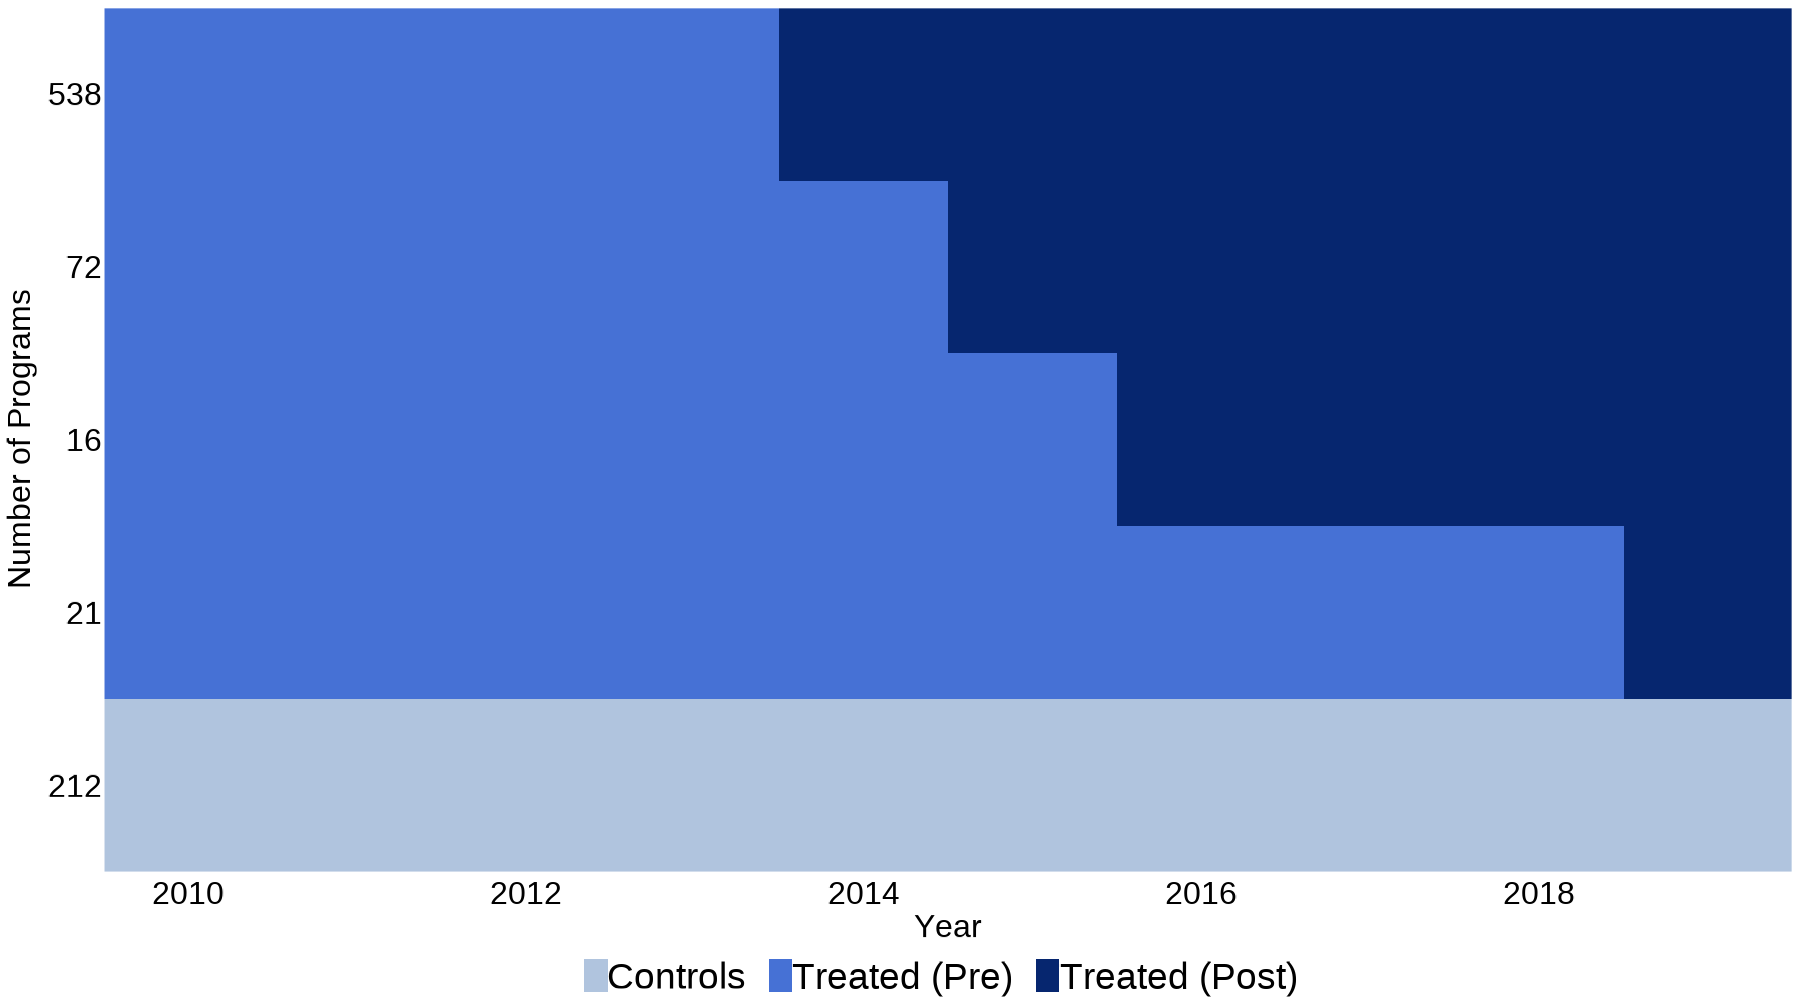
\includegraphics[width=\linewidth]{figures/desc-timing.png}
    \hfill
\caption*{\footnotesize{\textit{Notes:} The figure summarizes the treatment structure of the sample, where the unit of observation is a residency program (institution) and the treatment is the host state's adoption of Medicaid expansion. Programs are grouped by the timing of their state's expansion, and the vertical axis reports the number of programs in each group. Medium-blue cells denote treated programs in years before their state expanded Medicaid (``Treated (Pre)''), dark-navy cells denote treated programs in expansion and post-expansion years (``Treated (Post)''), and light-blue cells denote never-expansion (control) programs. The horizontal axis is the calendar year. The figure illustrates the staggered rollout of Medicaid expansion exploited by the difference-in-differences design. Data are from NRMP Main Residency Match reports, 2010--2019. The plot is produced with the \texttt{panelview} package (Mou, Liu, and Xu).}}
\end{figure}

\begin{figure}[H]
    \caption{Total Matched Residency Positions by Expansion Cohort}
    \label{fig2}
    \centering
      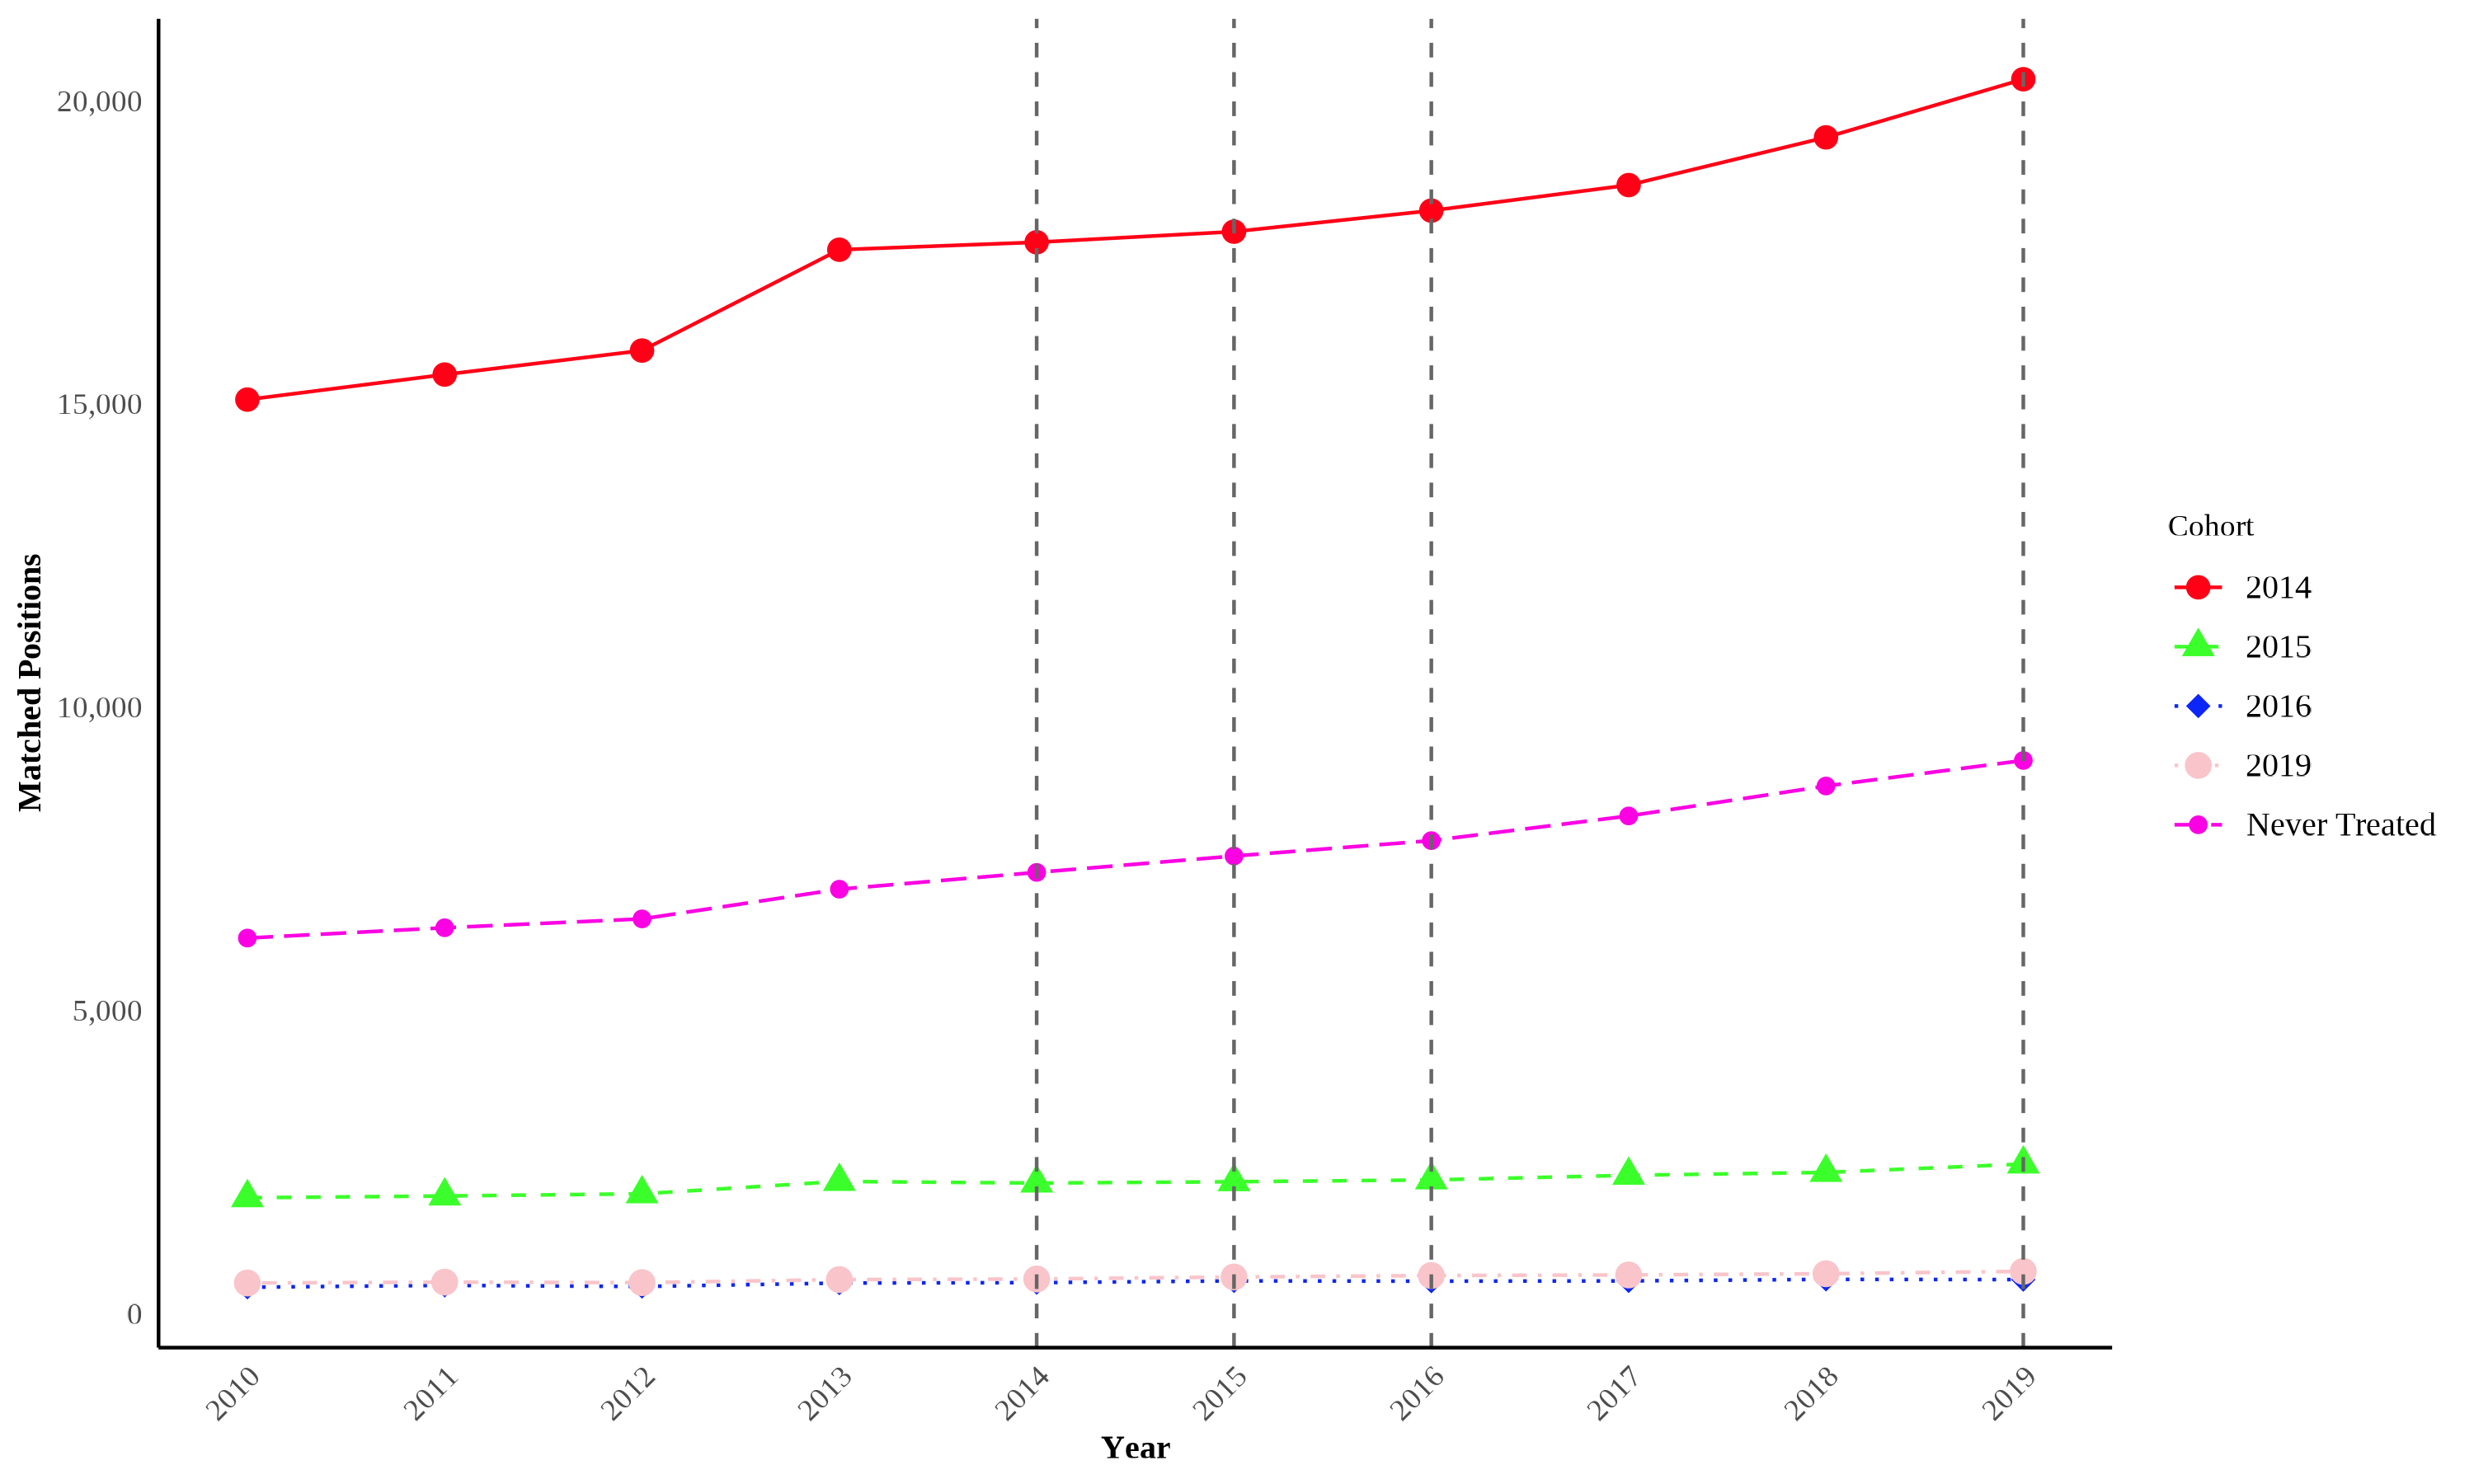
\includegraphics[width=\linewidth]{figures/desc-cohort-levels.png}
    \hfill
\caption*{\footnotesize{\textit{Notes:} The figure plots the total number of matched residency positions by year, separately for each Medicaid-expansion cohort. A cohort is defined by the calendar year in which a program's state expanded Medicaid (2014, 2015, 2016, and 2019); programs in states that never expanded over the sample period are grouped as ``Never Treated.'' Each series sums matched positions across all programs in the cohort, where positions are first aggregated to the institution-year level across specialties. Dashed vertical lines mark the expansion years of the treated cohorts. The figure is descriptive and is not adjusted for fixed effects or covariates. Data are from NRMP Main Residency Match reports, 2010--2019.}}
\end{figure}

\begin{figure}[H]
    \caption{Matched Residency Positions per 100,000 Population by Expansion Cohort}
    \label{fig3}
    \centering
      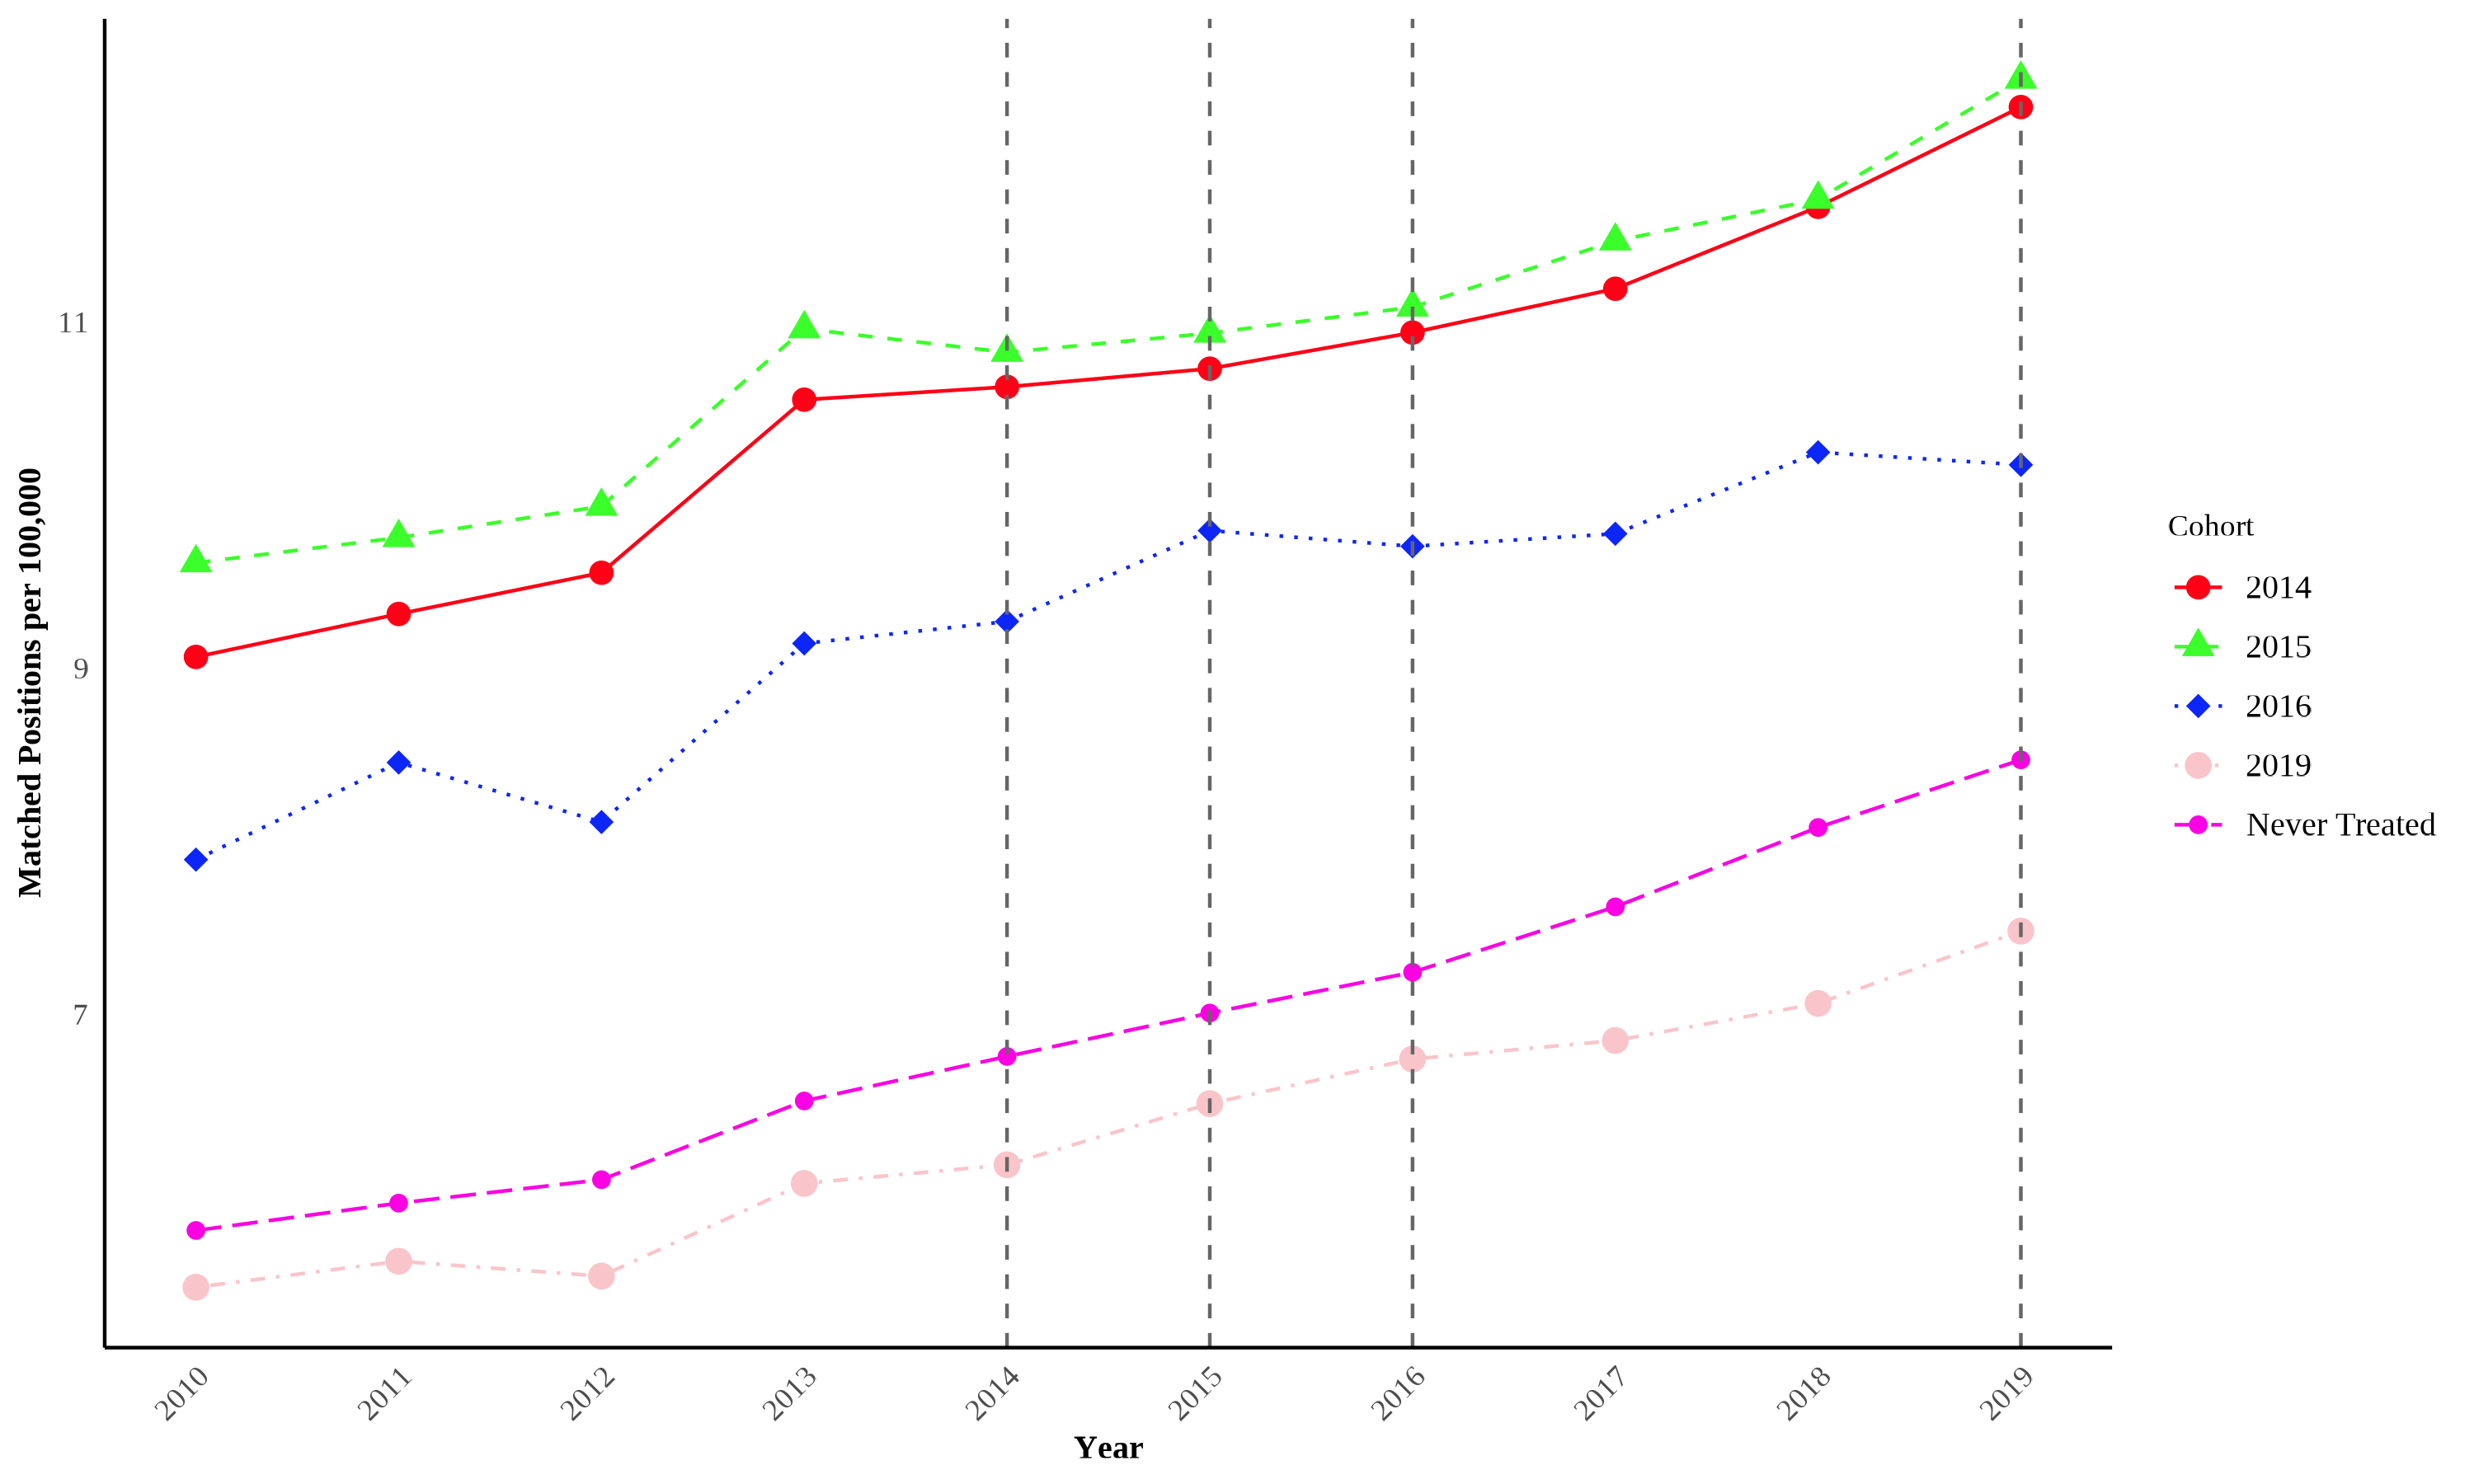
\includegraphics[width=\linewidth]{figures/desc-cohort-percapita.png}
    \hfill
\caption*{\footnotesize{\textit{Notes:} The figure plots matched residency positions per 100,000 population by year, separately for each Medicaid-expansion cohort. Cohorts are defined by the calendar year in which a program's state expanded Medicaid (2014, 2015, 2016, and 2019), with programs in non-expansion states grouped as ``Never Treated.'' For each cohort and year, matched positions and population are summed across the cohort's states before computing the rate per 100,000, using 2010 state population. Dashed vertical lines mark the expansion years of the treated cohorts. The figure is descriptive and is not adjusted for fixed effects or covariates. Data are from NRMP Main Residency Match reports, 2010--2019, and U.S.\ Census Bureau state population estimates.}}
\end{figure}

\begin{figure}[H]
    \caption{Growth in Physicians per 100,000 Population Relative to Total Population}
    \label{fig4}
    \centering
      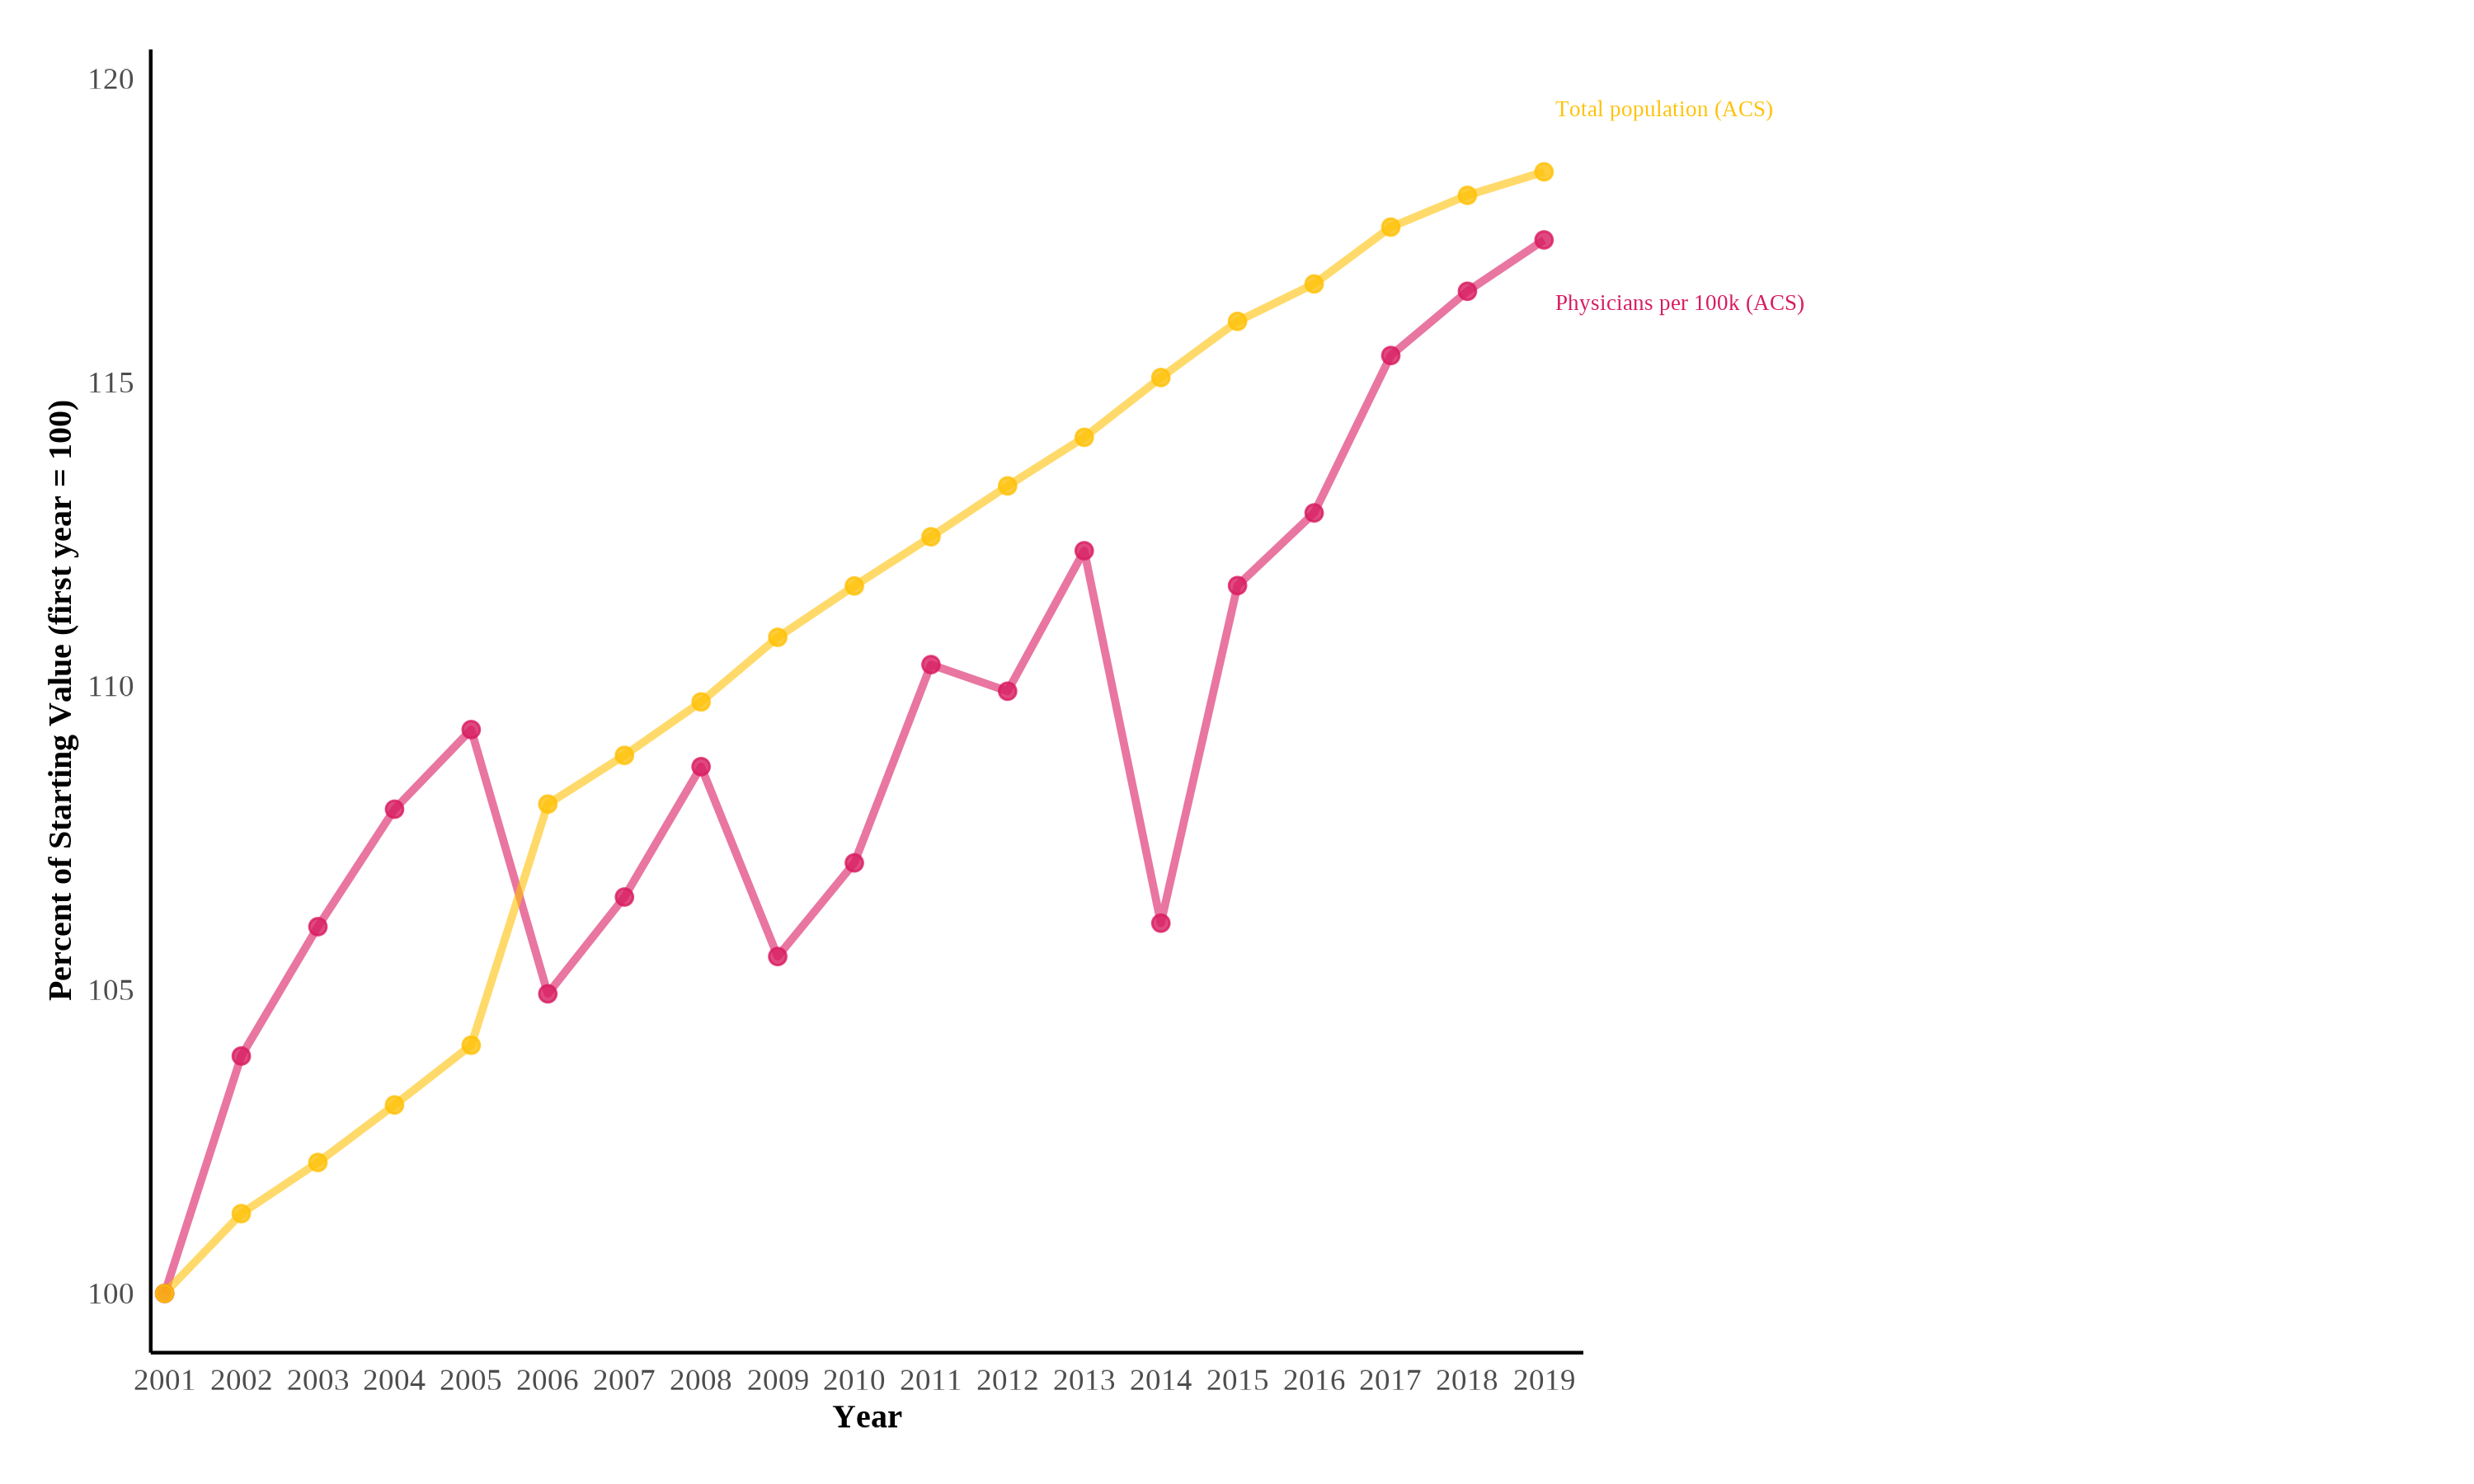
\includegraphics[width=\linewidth]{figures/desc-physician-growth.png}
    \hfill
\caption*{\footnotesize{\textit{Notes:} The figure plots the cumulative percent change since 2001 (2001 $= 100$) in two national series from the American Community Survey (ACS): physicians per 100,000 population and total population. Physicians are defined as employed workers in the harmonized occupation code for physicians and surgeons (\texttt{OCC1950} $= 75$). Estimates use the ACS person weight (\texttt{PERWT}). Data are from IPUMS-USA. The figure motivates the analysis by showing that the physician-to-population ratio has roughly tracked, rather than outpaced, population growth.}}
\end{figure}


\begin{figure}[H]
    \caption{Effect of Medicaid Expansion on Matched Residency Positions: Event Study Estimates}
    \label{fig5}
    \centering
      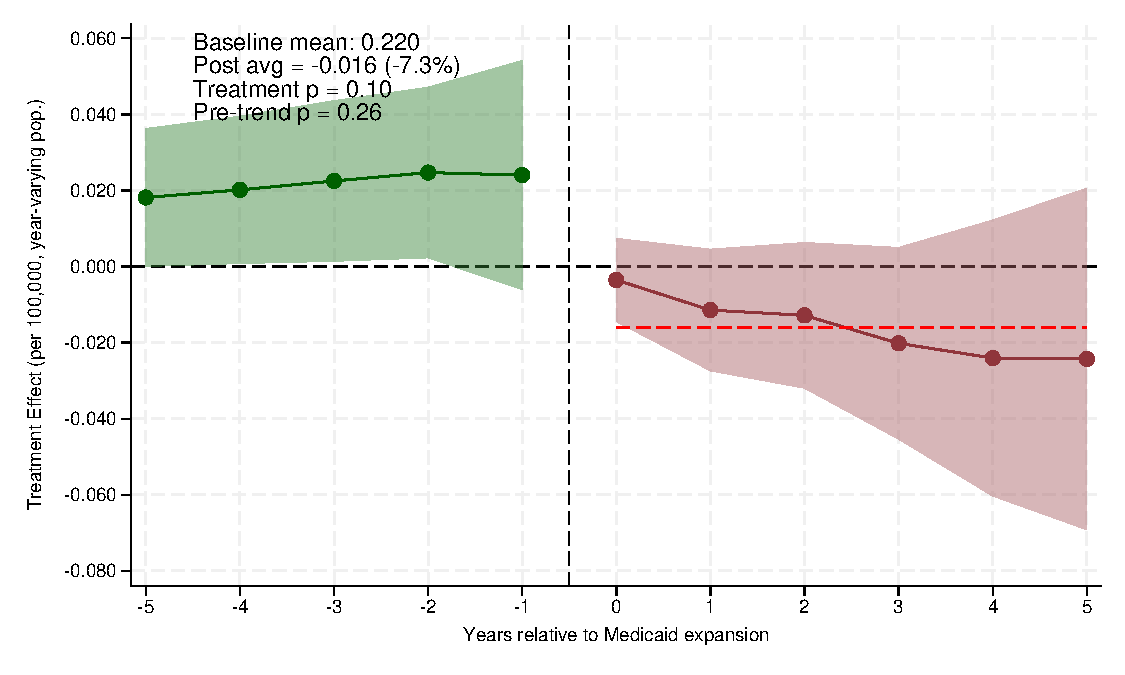
\includegraphics[width=\linewidth]{figures/main-headline.pdf}
    \hfill
\caption*{\footnotesize{\textit{Notes:} The figure plots event-study coefficients from the imputation estimator of Borusyak, Jaravel, and Spiess (2024), where the outcome is matched residency positions per 100,000 \emph{contemporary} (year-varying) state population from the American Community Survey. The horizontal axis measures years relative to a state's Medicaid expansion; year 0 is the first year of expansion. Green circles (years $-5$ to $-1$) show pre-expansion coefficients. Dark red circles (years $0$ to $+5$) show post-expansion treatment effects. The dashed red line indicates the average post-expansion treatment effect ($-0.016$), approximately $-7.3$ percent relative to the pre-expansion mean of $0.22$ matched positions per 100,000 (joint $p = 0.10$); the pre-expansion coefficients are jointly small and consistent with parallel trends (pre-trend $p = 0.26$). As discussed in the text, the aggregate magnitude is imprecise under randomization inference; the sign, dynamics, and mechanism are the robust features. Shaded bands are 95 percent confidence intervals. Regressions include hospital and year fixed effects and weight by 2010 state population. Standard errors are clustered at the state level.}}
\end{figure}

\newpage
\pagebreak

\begin{figure}[H]
    \caption{Effect of Medicaid Expansion on Direct GME (DGME) Payments: Event Study Estimates}
    \label{afig13}
    \centering
      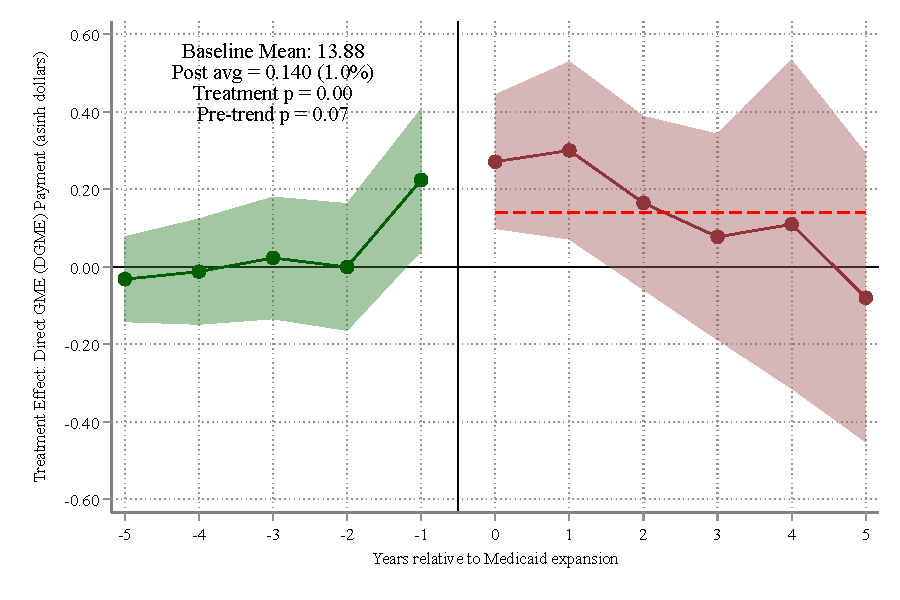
\includegraphics[width=\linewidth]{figures/main-firststage-dgme.pdf}
    \hfill
\caption*{\footnotesize{\textit{Notes:} The figure plots event-study coefficients from the imputation estimator of Borusyak, Jaravel, and Spiess (2024). The outcome is the inverse hyperbolic sine (asinh) of Direct GME (DGME) payments per teaching hospital, from CMS Medicare hospital cost reports; DGME reimburses the direct costs of residency training (resident salaries, benefits, and faculty supervision). Because $\operatorname{asinh}(x)\approx\ln(2x)$ for large $x$, coefficients approximate proportional changes. The sample comprises all hospitals receiving Medicare GME payments, observed at the hospital--fiscal-year level, with never-expansion states as the comparison group. The horizontal axis measures years relative to a state's Medicaid expansion; year 0 is the first year of expansion. Green circles (years $-5$ to $-1$) show pre-expansion coefficients; dark red circles (years $0$ to $+5$) show post-expansion treatment effects. The dashed red line indicates the average post-expansion effect of $0.140$, roughly a $14$ percent increase in DGME payments (joint $p < 0.01$), with the largest effects in the first two post-expansion years. Pre-expansion coefficients are near zero from event years $-5$ to $-2$; the elevated coefficient at $-1$ (joint pre-trend $p = 0.07$) is consistent with modest anticipatory increases in payments. Shaded bands are 95 percent confidence intervals. Estimates are based on 1,916 hospitals across 51 states and the District of Columbia. Regressions include hospital and year fixed effects and are unweighted. Standard errors are clustered at the state level.}}
\end{figure}

\newpage
\pagebreak

\begin{figure}[H]
    \caption{Effect of Medicaid Expansion on Indirect Medical Education (IME) Payments: Event Study Estimates}
    \label{afig14}
    \centering
      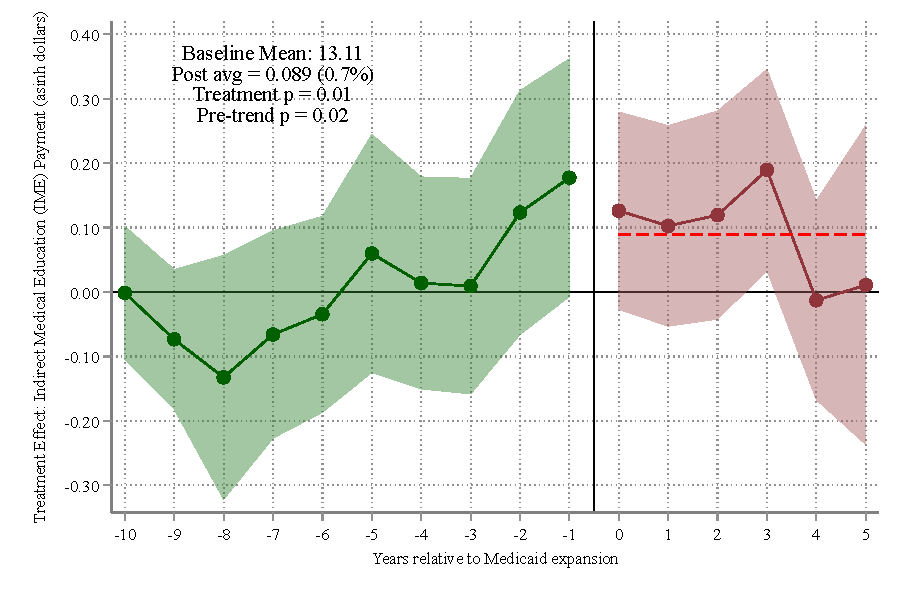
\includegraphics[width=\linewidth]{figures/main-firststage-ime.pdf}
    \hfill
\caption*{\footnotesize{\textit{Notes:} The figure plots event-study coefficients from the imputation estimator of Borusyak, Jaravel, and Spiess (2024) for the indirect component of GME payments, complementing the Direct GME estimate in \cref{afig13}. The outcome is the inverse hyperbolic sine (asinh) of Indirect Medical Education (IME) payments per teaching hospital, from CMS Medicare hospital cost reports; IME is the indirect operating-cost adjustment paid to teaching hospitals, as distinct from the direct training costs captured by DGME. Because $\operatorname{asinh}(x)\approx\ln(2x)$ for large $x$, coefficients approximate proportional changes. The average post-expansion effect is $0.059$, roughly a $6$ percent increase, and is only marginally significant (joint $p = 0.06$); pre-expansion coefficients are jointly insignificant (joint pre-trend $p = 0.32$). The muted response relative to Direct GME indicates that the GME-financing effect of expansion operates primarily through direct resident-training payments rather than the indirect adjustment. The sample comprises all hospitals receiving Medicare GME payments at the hospital--fiscal-year level, with never-expansion states as the comparison group. Green circles (years $-5$ to $-1$) show pre-expansion coefficients; dark red circles (years $0$ to $+5$) show post-expansion treatment effects. Shaded bands are 95 percent confidence intervals. Estimates are based on 1,916 hospitals across 51 states and the District of Columbia. Regressions include hospital and year fixed effects and are unweighted. Standard errors are clustered at the state level.}}
\end{figure}

\newpage
\pagebreak

\begin{figure}[H]
    \caption{Mechanism: Effect of Medicaid Expansion by State Medicaid GME Formula}
    \label{fig:mech_gme}
    \centering
    \begin{subfigure}{\linewidth}
        \centering
        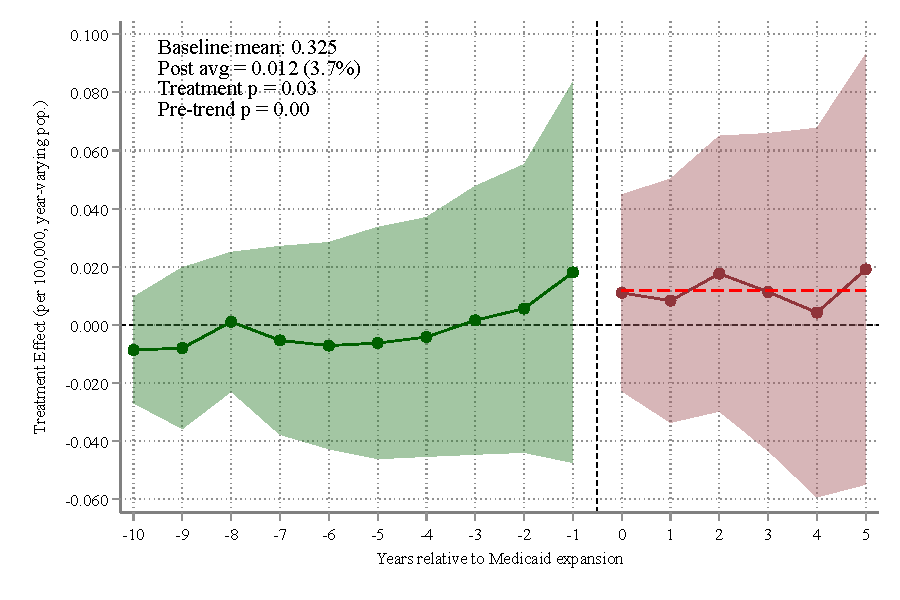
\includegraphics[width=0.75\linewidth]{figures/main-mechanism-volume.pdf}
        \caption{Volume-Responsive GME States}
        \label{fig:mech_gme:vol}
    \end{subfigure}
    \hfill
    \begin{subfigure}{\linewidth}
        \centering
        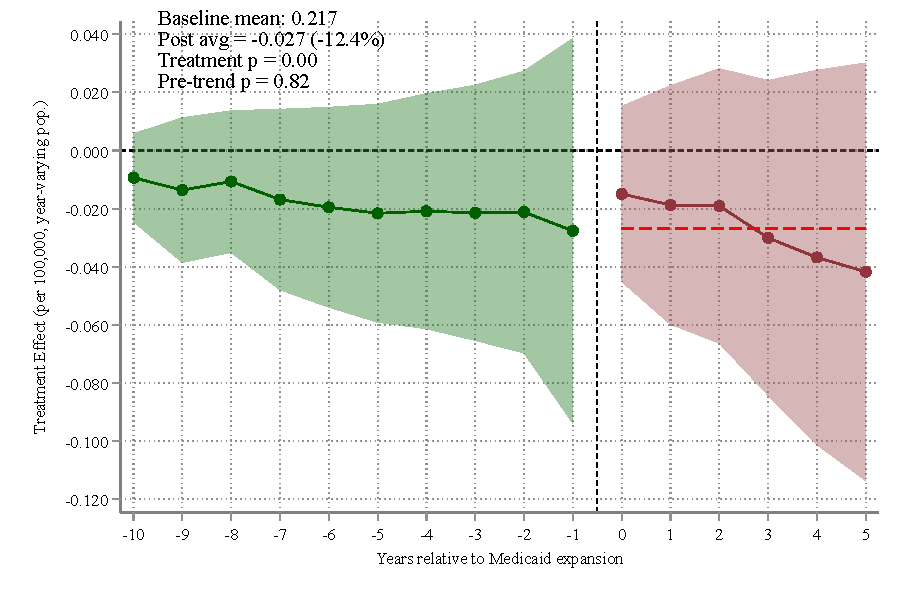
\includegraphics[width=0.75\linewidth]{figures/main-mechanism-nonresp.pdf}
        \caption{Non-Responsive GME States (Fixed/None)}
        \label{fig:mech_gme:nonresp}
    \end{subfigure}
\caption*{\footnotesize{\textit{Notes:} The figure plots event-study coefficients
from the imputation estimator of \textcite{borusyak2024revisiting}, estimated
separately for expansion states with volume-responsive (top) versus non-responsive
(bottom) Medicaid GME formulas, each using non-expansion states as the comparison
group. The outcome is matched residency positions per 100{,}000 contemporary
(year-varying) state population. In non-responsive states the average post-expansion
effect is $-0.022$ (an $11.7$ percent decline; joint $p < 0.01$) following flat
pre-expansion coefficients (pre-trend $p = 0.15$); in volume-responsive states it is
$+0.013$ ($+3.4$ percent), with no decline. A pooled interacted model puts the
volume-minus-non-responsive difference in average post effects at $0.035$ per
100{,}000 (clustered p $< 0.001$; randomization-inference p $= 0.19$). The
volume-responsive panel exhibits a pronounced upward pre-trend (pre-trend
$p < 0.001$), so its estimate should be read with caution; the non-responsive
contraction is the more robust leg of the comparison.
Volume-responsive states reward higher Medicaid volume with larger GME payments, so
expansion mechanically raises GME revenue; non-responsive states (fixed per-resident
amounts, lump-sum grants, or no Medicaid GME) gain none. States are classified from
the Medicaid GME payment methodology reported in \textcite{henderson2013}. Green
circles (years $-5$ to $-1$) show pre-expansion coefficients; dark red circles
(years $0$ to $+5$) show post-expansion treatment effects; the dashed red line marks
the average post-expansion effect. Shaded bands are 95 percent confidence intervals.
Regressions include hospital and year fixed effects, are weighted by state
population. Standard errors are clustered at the state level.}}
\end{figure}

\begin{figure}[H]
    \caption{Effect of Medicaid Expansion on Matched Residency Positions by Hospital Location: Event Study Estimates}
    \label{fig6}
    \centering
      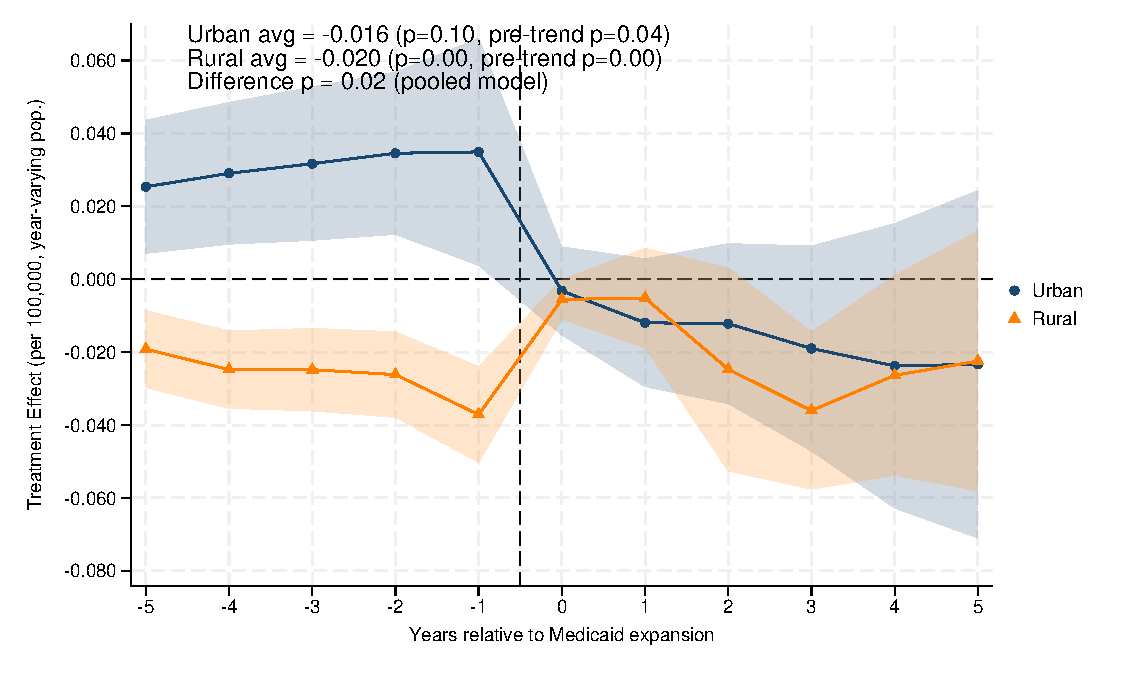
\includegraphics[width=\linewidth]{figures/main-location.pdf}
    \hfill
\caption*{\footnotesize{\textit{Notes:} The figure plots event-study coefficients from the imputation estimator of Borusyak, Jaravel, and Spiess (2024), estimated in two split-sample regressions for urban (blue circles) and rural (orange triangles) hospitals; each subsample keeps the never-expansion hospitals of its own type as the comparison group, so each series carries its own pre-expansion path and pre-trends test. Urban hospitals are those in counties with 2010 RUCA codes 1--3; rural hospitals are those with RUCA codes above 3. The outcome is matched positions per 100,000 contemporary (year-varying) population. The horizontal axis measures years relative to a state's Medicaid expansion; year 0 is the first year of expansion. The average post-expansion treatment effect is $-0.016$ for urban hospitals (joint p $= 0.10$; pre-trend p $= 0.04$, with uniformly positive pre-expansion coefficients) and $-0.020$ for rural hospitals (joint p $< 0.001$). The rural subsample fails its own pre-trends test (p $< 0.001$), with negative pre-expansion coefficients comparable in size to the post-expansion effects, so the rural series should be read descriptively. A pooled interacted model puts the urban--rural difference in average post effects at $-0.014$ (p $= 0.02$), but that model shares pre-trends across groups. Shaded bands are 95 percent confidence intervals. Regressions include hospital and year fixed effects and weight by 2010 state population. Standard errors are clustered at the state level.}}
\end{figure}

\begin{figure}[H]
    \caption{Effect of Medicaid Expansion on Matched Residency Positions by Specialty Type: Event Study Estimates}
    \label{fig7}
    \centering
    \begin{subfigure}{\linewidth}
        \centering
        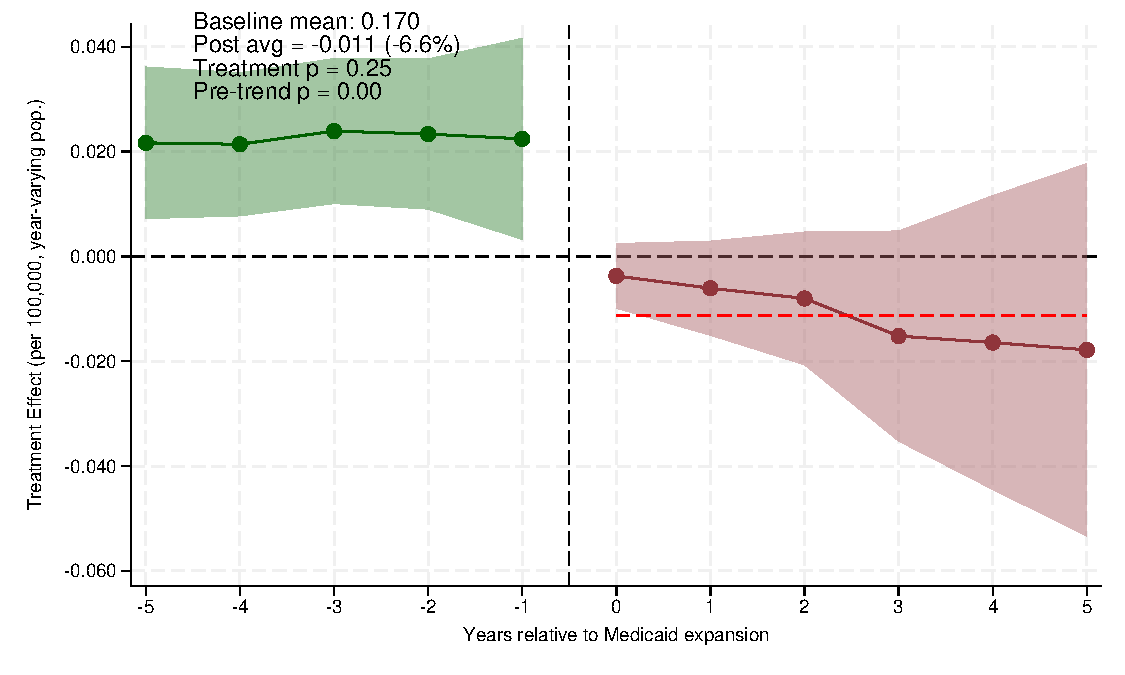
\includegraphics[width=0.75\linewidth]{figures/main-specialty-nonprimary.pdf}
        \caption{Non-Primary Care Positions}
        \label{fig7:non-prim-care}
    \end{subfigure}
    \hfill
    \begin{subfigure}{\linewidth}
        \centering
        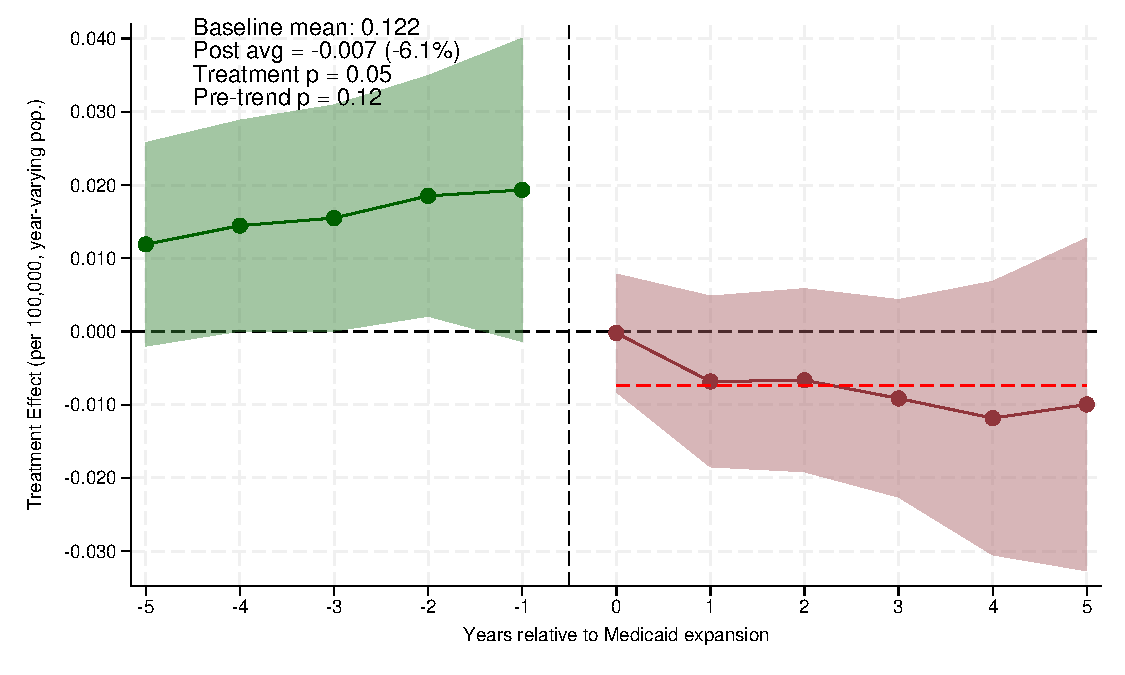
\includegraphics[width=0.75\linewidth]{figures/main-specialty-primary.pdf}
        \caption{Primary Care Positions}
        \label{fig7:prim-care}
    \end{subfigure}
\caption*{\footnotesize{\textit{Notes:} The figure plots event-study coefficients from the imputation estimator of Borusyak, Jaravel, and Spiess (2024) estimated separately for non-primary care (top panel) and primary care specialties (bottom panel). Primary care includes family medicine, internal medicine, and pediatrics. The outcome is matched positions per 100,000 contemporary (year-varying) population. The horizontal axis measures years relative to a state's Medicaid expansion; year 0 is the first year of expansion. For non-primary care programs, the average post-expansion treatment effect is $-0.002$ ($-4.7$ percent; p $= 0.22$; pre-trend $p = 0.01$). For primary care programs, it is $-0.003$ ($-4.6$ percent; p $= 0.06$; pre-trend $p = 0.06$). Both panels exhibit differential pre-trends, so the specialty estimates should be read as suggestive. Shaded bands are 95 percent confidence intervals. Regressions include hospital and year fixed effects and weight by 2010 state population. Standard errors are clustered at the state level.}}
\end{figure}

\begin{figure}[H]
    \caption{Robustness of Event Study Estimates Across Difference-in-Differences Estimators: Matched Residency Positions per 100,000 Population}
    \label{fig8}
    \centering
      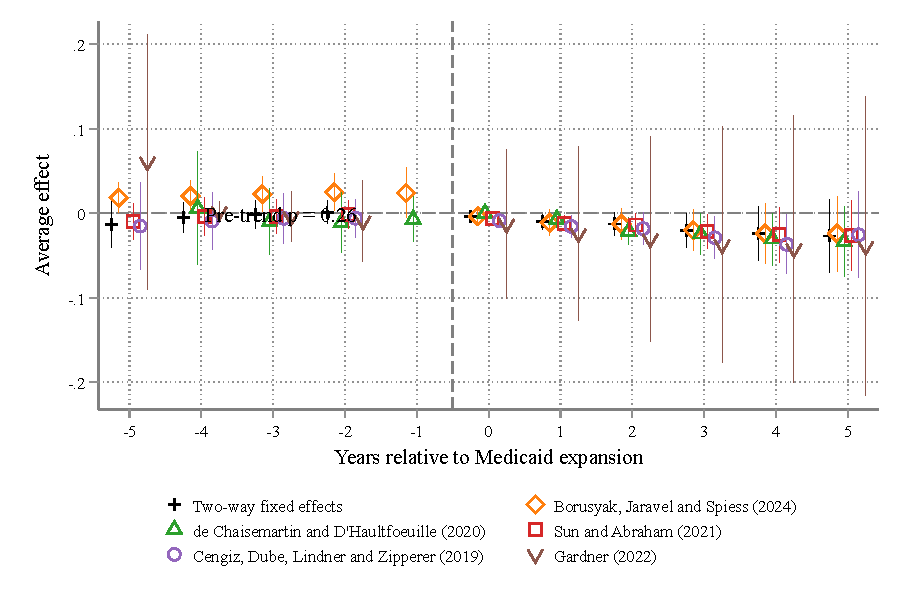
\includegraphics[width=\linewidth]{figures/main-estimators.pdf}
    \hfill
\caption*{\footnotesize{\textit{Notes:} The figure compares event-study estimates of the effect of Medicaid expansion on matched residency positions per 100,000 contemporary (year-varying) population across six difference-in-differences estimators that are robust to treatment-effect heterogeneity under staggered adoption: two-way fixed effects; Borusyak, Jaravel, and Spiess (2024); de Chaisemartin and D'Haultfoeuille (2020); Sun and Abraham (2021); Cengiz, Dube, Lindner, and Zipperer (2019); and Gardner (2022). The heterogeneity-robust estimator of Callaway and Sant'Anna (2021) is excluded because it is not well identified in the sparsely populated never-treated cells of this sample. The pre-trend $p$-value reported in the panel is from the Borusyak, Jaravel, and Spiess (2024) estimator. The horizontal axis measures years relative to a state's Medicaid expansion; the dashed vertical line marks the expansion year. Regressions include hospital and year fixed effects and weight by 2010 state population. Standard errors are clustered at the state level.}}
\end{figure}

\clearpage
